\documentclass[5p,times]{elsarticle}

\usepackage{booktabs}
\usepackage{comment}
\usepackage{amsmath}
\usepackage{listings}
\usepackage{hyperref}
\usepackage{cleveref}
\usepackage[normalem]{ulem}
\newtheorem{example}{Example}
\newtheorem{definition}{Definition}
\newtheorem{formula}{Formula}
\crefname{lstlisting}{listing}{listings}
\Crefname{lstlisting}{Listing}{Listings}
\crefname{example}{example}{example}
\Crefname{example}{Example}{Example}
\newtheorem{req}{Requisite}

% \newcounter{example}[section]
% \newenvironment{example}[1][]{ \refstepcounter{example}\par\medskip
%   \noindent \fontfamily{lmss}\selectfont \textbf{EXAMPLE~\theexample. #1}} 
   
\newcommand{\gp}[1]{{\color{red}{\textbf{#1}}}}
\newcommand{\gpc}[2]{{\color{red}{\textbf{#1}}} {\color{blue}\sout{#2}}}
\newcommand{\jg}[1]{{\color{orange}{\textbf{#1}}}}
\newcommand{\jgc}[2]{{\color{orange}{\textbf{#1}}} {\color{blue}\sout{#2}}}
\newcommand{\mf}[1]{{\color{blue}{\textbf{#1}}}}
\newcommand{\mfc}[2]{{\color{blue}{\textbf{#1}}} {\color{blue}\sout{#2}}}
   

\begin{document}

\sloppy

\begin{frontmatter}
%%
%% The "title" command
\title{HAMLET: Human-centric AutoMl via Logic and argumEnTation}
%%
%% The "author" command and its associated commands are used to define
%% the authors and their affiliations.
% \author{Joseph Giovanelli}
% \orcid{0000-0002-0990-3893}
% \affiliation{%
%   \institution{\textsc{ALMA MATER STUDIORUM} --- Università di Bologna}
% }
% \email{j.giovanelli@unibo.it}

% \author{Giuseppe Pisano}
% \orcid{0000-0003-0230-8212}
% \affiliation{%
%   \institution{\textsc{ALMA MATER STUDIORUM} --- Università di Bologna}
% }
% \email{g.pisano@unibo.it}

\author{Matteo Francia}\ead{m.francia@unibo.it}
\author{Joseph Giovanelli\corref{cor1}}\ead{j.giovanelli@unibo.it}
\author{Giuseppe Pisano}\ead{g.pisano@unibo.it}
\cortext[cor1]{Corresponding author}
\address{DISI -- University of Bologna, Italy}
% \cortext[cor1]{Corresponding author}
% \author[1]{Joseph Giovanelli}[%
% orcid=0000-0002-0990-3893,
% email=j.giovanelli@unibo.it,
% ]
% \author[1]{Giuseppe Pisano}[%
% orcid=0000-0003-0230-8212,
% email=g.pisano@unibo.it,
% ]
% \address[1]{\textsc{ALMA MATER STUDIORUM} --- Università di Bologna}

%%
%% The abstract is a short summary of the work to be presented in the
%% article.
\begin{abstract}
In the last decade, we have witnessed an exponential growth in both the complexity and the number of Machine Learning (ML) techniques.
As a consequence, leveraging such methods to solve real-case problems has become difficult for a Data Scientist (DS).
Automated Machine Learning (AutoML) tools were devised to alleviate that task, but easily became as complex as the ML techniques themselves.
The DS has started to rely on this kind of tools without understanding their functioning, thus loosing the control over the process.

In this vision paper, we propose HAMLET (Human-centric AutoMl via Logic and Argumentation), a framework that would help the DS to redeem her centrality.
HAMLET is inspired to the well-known standard process model CRISP-DM.
Iteration after iteration, the knowledge is augmented by acquiring more constraints about the problem until a suitable solution is found.
HAMLET leverages Logic and Argumentation to merge both constraints and solutions in an uniformed human- and machine-readable medium.
Not only it allows an easy exploration of the new knowledge at each iteration, but it also enforces a continuous revision via the AutoML tool and the confrontation between the DS and Domain Experts.
\end{abstract}

%%
%% Keywords. The author(s) should pick words that accurately describe
%% the work being presented. Separate the keywords with commas.
\begin{keyword}
  AutoML, Logic, Argumentation, CRISP-DM, Data Scientist
\end{keyword}

\end{frontmatter}
%%
%% This command processes the author and affiliation and title
%% information and builds the first part of the formatted document.
% \maketitle

%%%%%%%%%%%%%%%%%%%%%%%%%%%%%%%%%%%%%%%%%%%%%%%%%%%%%%%%%%%
\section{Introduction}\label{intro}
%%%%%%%%%%%%%%%%%%%%%%%%%%%%%%%%%%%%%%%%%%%%%%%%%%%%%%%%%%%

In relation to data platforms, it is well-known that Machine Learning (ML) plays a key role in the process of data analysis.
As a matter of fact, it has been pervasively employed to cope with each and every type of real-case problems \cite{zhou2017ml, dataplat2, francia2021moses, multi-store}.
The Data Scientist (DS) (i.e., a specialist of data analysis) starts by collecting raw data in an arbitrary format. 
Then she typically leverages a process model that will help her to translate the \textit{knowledge} about the problem into \textit{ML constraints}, and deploy the \textit{solution}.
CRISP-DM \cite{wirth2000crisp} is the most acknowledged standard process model and we will take it as a reference in the whole paper.
A solution consists of a \textit{ML pipeline}: a series of \textit{Data Pre-processing transformations} and a \textit{ML algorithm}.
The DS can instantiate both with a large set of \textit{techniques}, which have their own tunable hyper-parameters.
These choices highly affect the performance of a solution.

Automated Machine Learning (AutoML) tools have been devised with the aim of assisting the DS during the ML pipeline instantiation.
They leverage state-of-the-art optimisation approaches to smartly explore huge search spaces of solutions. %(i.e., ML pipelines with different techniques and hyper-parameters). 
AutoML has been demonstrated to provide accurate \textit{performance}, even in a limited time budget.
During the setting up of the search space, it is highly important to the DS to leverage the knowledge about the problem, considering all the ML constraints. %(i.e., \textit{domain-related}, \textit{data-related}, \textit{transformation-related}, and \textit{algorithm related}). 
%\jg{I am not sure if I would mention the kind of constraints without explaining what they are}
Otherwise, it might lead the AutoML tool to retrieve \textit{invalid solutions} (i.e., the \textit{result} of those cannot be deemed \textit{correct}).
Besides, AutoML tools became that complex to make it difficult for the DS to understand their functioning, hence losing the control over the process.
Researchers are aware of these problems \cite{XinWLSP21automationml}.
There are some works that have prescribed to use a human-centric framework for AutoML \cite{gil2019towards, lee2020human, wang2019human}, yet suggesting only design requirements. 
Alternatively, the authors in \cite{ono2020pipelineprofiler} have proposed a tool that visualises the best and the worst solutions retrieved by an AutoML tool.
%However, they do not put any effort in providing a framework that merges AutoML inputs -- i.e., constraints -- with outputs---i.e., solutions.

We claim that the need of a human-centric framework for AutoML is real, and it is crucial for the DS to \textit{augment} her knowledge via the retrieved solutions.
%overcome these problems and give to the DS full control on the data.
At this purpose we propose HAMLET (Human-centric AutoMl via Logic and Argumentation), which leverages Logic and Argumentation to:
\begin{itemize}
    \item structure the ML constraints and the AutoML solutions in a Logical Knowledge Base (LogicalKB);
    \item parse the structured LogicalKB into a human- and machine-readable medium called Problem Graph;
    \item leverage the Problem Graph to set up an AutoML search space;
    \item leverage the Problem Graph to allow both the DS and an AutoML tool to revise the current knowledge.
\end{itemize}
\Cref{fig:approach} illustrates how CRISP-DM, AutoML, and HAMLET interact with each other.
We remark that our framework allows the DS to never loose the control over the process, and hence her centrality. 
Besides, HAMLET allows to visualise the knowledge in an human- and machine-readable format.
%Here it was DSs
As advocated in \cite{drozdal2020trust}, the DS requires to understand the AutoML process in order to trust the proposed solutions.

The remain of the paper is structured as follows.
\Cref{automl} and \Cref{logic} introduce the main notions of respectively AutoML and Argumentation.
\Cref{towards} illustrates our framework.
Finally, \Cref{concl} draws the conclusions and potential leveraging.

%%%%%%%%%%%%%%%%%%%%%%%%%%%%%%%%%%%%%%%%%%%%%%%%%%%%%%%%%%%
\section{AutoML}\label{automl}
%%%%%%%%%%%%%%%%%%%%%%%%%%%%%%%%%%%%%%%%%%%%%%%%%%%%%%%%%%%

AutoML tools have been conceived with the aim of lightening the DS in the overwhelming practise of finding the suitable solution for the case at hand.
We recall that in the context of data platforms, a solution is a ML pipeline, defined as a series of Data Pre-processing transformations followed by a ML algorithm.
In its early days, only the instantiation of the latter -- the ML algorithm -- was addressed.
Auto-Weka \cite{kotthoff2019auto} formalised the problem as Combined Algorithm Selection and Hyper-parameter Optimisation (CASH).
In a nutshell, in order to find the most performing configuration, various ML algorithms -- and related hyper-parameters -- have to be tested over a dataset.
Such a problem was successfully coped by leveraging Bayesian Optimisation (BO) \cite{frazier2018tutorial}, a sequential design strategy for global optimisation.
The process involves several iterations, through which different configurations are explored. %during which configurations are explored.
As the iterations advance, an increasingly accurate model is built on top of the previous explored configurations, with the aim of suggesting the most promising ones.
The configurations keep being explored, and updating the model, until a budget in terms of either iterations or time is reached.
%The configurations keep being explored, and thus to update the model, until a budget in terms of either iterations or time is reached.

Recently, AutoML is no longer limited to optimise just the ML algorithm phase, but it includes Data Pre-processing as well.
Indeed, with the aid of a series of transformations, it is possible to achieve better performance, unattainable with the most performing ML algorithm configuration \cite{giovanelli2021effective}. %dolap mio
In \cite{quemy2019data}, the author formalised the problem as Data Pipeline Selection and Optimisation (DPSO). %dolap quemy
Each of the transformations can be instantiated with different techniques, which -- analogously to the ML algorithms -- have their own hyper-parameters.
Auto-sklearn \cite{feurer2019auto} includes Data Pre-processing already in its first versions. %auto-sklearn
Yet, they fix the arrangement of the transformations a priori, without considering that the most performing arrangement changes according to the case and data at hand.
Considering several arrangements translates into larger search spaces, not easy to explore.
%Fortunately, there are some other tools that take into accounts also such arrangements \cite{olson2016tpot}. %tpot

In order to cope with ever larger research spaces, various expedients have been employed.
Meta-learning (i.e., learning on top of learning) has been used to warm-start the Bayesian Optimisation (i.e., to boost the convergence process) by suggesting promising configurations (i.e., that worked well in previous similar real-case problems) \cite{giovanelli2021data}. %auto-sklearn, MLSMART, is mio
Ensembling (i.e., construction of a high-performing solution combining several low-performing solutions; e.g., bagging, boosting, stacking) have been leveraged to enable AutoML tools to retrieve a solution that combines the best performing configurations, instead of retrieving just the best performing one \cite{feurer2019auto}. %auto-sklearn h2o
Moreover, multi-fidelity methods (i.e., the use of several partial estimations to boost the time-consuming evaluation process) have been exploited to let AutoML tools explore as many configurations as possible.

All in all, the improvements made over the last years have yielded to be so substantial that AutoML is nowadays able to handle the entire ML pipeline instantiation.
Yet, the stacking of complex mechanisms on top of each other unavoidably led to a less understanding of the process by the DS.
%We claim that she has a key role in it, because of her awareness about all the constraints of the problem.
%Some constraints are derived by the domain (e.g., a solution may be based on some correlations considered spurious), others are intrinsic in the data (e.g., some features can be semantically misinterpreted).
%Still, there are constraints related to the concatenation of the transformations in the Data Pre-processing stage, others related to the chosen ML algorithm, and last but not least, some constraints regard an ethical perspective.
We believe that the DS has the duty to revise and supervise the suggested solutions.
Unfortunately, state-of-art AutoML tools overlook her role, and do not let that possible.

\begin{figure*}
    \centering
    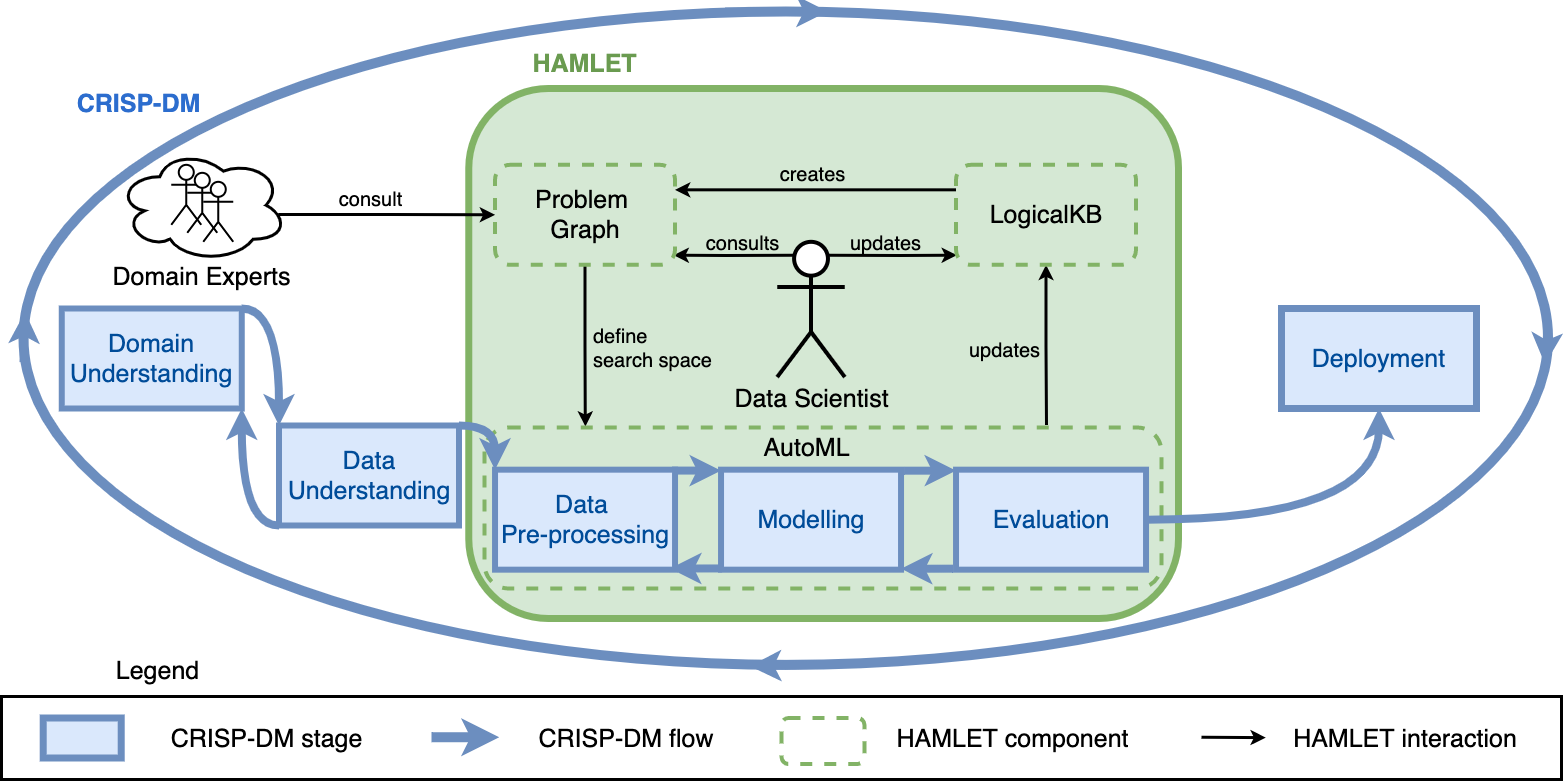
\includegraphics[width=0.85\textwidth]{img/dymmymodel.png}
    \caption{Integration of the HAMLET framework with the CRISP-DM standard process model and AutoML.}
    \label{fig:approach}
\end{figure*}

%%%%%%%%%%%%%%%%%%%%%%%%%%%%%%%%%%%%%%%%%%%%%%%%%%%%%%%%%%%
\section{Logic \& Argumentation}\label{logic}
%%%%%%%%%%%%%%%%%%%%%%%%%%%%%%%%%%%%%%%%%%%%%%%%%%%%%%%%%%%

% Formal logic in its actual form emerged from philosophy in the nineteenth century as the abstract study of statements, sentences and deductive arguments \cite{Paulson2018logichistory}. The final goal was to determine the validity of these elements just by examining the structures or logical forms that they embody, without considering their actual meaning or content. We can summarise logic as the definition and study of structured languages, which enables an unambiguous manipulation and a clear test of the validity of the statements expressed in those languages.

% For example, we can define a logical formalism as a precisely defined symbolic language that includes logical primitives such as ``and'', ``or'', ``not'', \ldots, and a series of rules for making logical deductions (e.g., \textit{modus ponens} \cite{susanne02mp}). Given a formalism of this type, it will be then possible to define a proof theory to determine the validity of statements expressed in it. Computational logic is the use of computers to automatise this procedure \cite{Paulson2018logichistory}.

Logic can be defined as the abstract study of statements, sentences and deductive arguments \cite{Paulson2018logichistory}.
From its birth, it has been developed and improved widely and now includes a variety of formalisms and technologies. Between all, Argumentation has proved itself an important tool for handling conflicting information (e.g., opinions, empirical data).
This has led to a great number of researches trying to establish a computational model of logical arguments.
%One of the most influential systems, proposed by Dung in his seminal work \cite{Dung1995abstractArg}, provides many insights into the nature of Argumentation, and it has led to a large number of works that have explored properties and developments of it \cite{besnardCL20argsurvey}.

In Abstract Argumentation \cite{Dung1995abstractArg}, a scenario can be represented by a directed graph. Each node represents an argument, and each edge denotes an attack by one argument to another. Each argument is regarded as atomic. There is no internal structure to an argument. Also, there is no specification of what is an argument or an attack. A graph can then be analysed to determine which arguments are acceptable according to some general criteria (i.e., semantics) \cite{baroniCG11semantics}.

A way to link Abstract Argumentation and logical formalisms has been advanced in the field of Structured Argumentation \cite{BesnardGHMPST14structured}, where we assume a formal logical language for representing knowledge (i.e., a Logical Knowledge Base), and specifying how arguments and conflicts (i.e., attacks) can be derived from that knowledge. 
In the structured approach, premises and claims of the argument are made explicit, and the relationship between them is formally defined through rules internal to the formalism. We can build the notion of attack as a binary relation over structured arguments that denotes when one argument is in conflict with another (e.g., contradictory claims or premises).
One of the main frameworks for Structured Argumentation is ASPIC\textsuperscript{+}\cite{Modgil2014aspic+}. In this formalism arguments are built with two kinds of inference rules: strict rules, whose premises guarantee their conclusion, and defeasible rules, whose premises only create a presumption in favour of their conclusion. 
Then conflicts between arguments can arise from both \textit{inconsistencies} in the Logical Knowledge Base and the defeasibility of the reasoning steps in an argument (i.e., a defeasible rule used in reaching a certain conclusion from a set of premises can also be attacked).
%Anyway, one of the most important features of the framework -- similarly to others formalisms \cite{Toni2014aba} in the Structured Argumentation field -- is the freedom that gives to users in the definition of the founding logical language to adopt. In this sense ASPIC\textsuperscript{+} can be seen not as a final framework but as a formalism to define custom Argumentation frameworks that satisfy a set of formal properties (e.g., logical consistency and closure postulates).

%Here it was DSs
In our view, once defined the right logical language for encoding the DS and AutoML knowledge, a Structured Argumentation model (e.g., an ASPIC\textsuperscript{+} instance \cite{arg2p-jlc}) would provide us with the formal machinery to build an Argumentation framework upon the data, while Abstract Argumentation would dispense the evaluation tools.

%%%%%%%%%%%%%%%%%%%%%%%%%%%%%%%%%%%%%%%%%%%%%%%%%%%%%%%%%%%
\section{Towards a human-centric approach}\label{towards}
%%%%%%%%%%%%%%%%%%%%%%%%%%%%%%%%%%%%%%%%%%%%%%%%%%%%%%%%%%

%Highly simplifying, the task of the DS is to find a performing solution, considering all the constraints that may apply to a ML problem.
Addressing ML problems encompasses the DS seeking for a solution, considering all the constraints of the case.
She usually leverages a process model as CRISP-DM.
%There are no universal well-defined practices to address such a task, which translates to the DS manually evaluating different ML pipelines, until a \textit{performing} and \textit{correct} one is found.
%However, DS have devised common practices to help in the process. 
% In \Cref{intro} we mentioned CRISP-DM, a standard process model that helps to structure the knowledge about the problem and not to be overwhelmed by its overall complexity. %find the correct solution.
% We believe that a closer analysis of this methodology is necessary for two main reasons. 
% First of all, it gives an excellent example on the centrality of the DS and on the essential importance of enriching her knowledge across the process.
% Second of all, the analysis will provide the reader with instruments to better understand the issues that the resolution of a ML problem involves. %in AutoML techniques and define which issues our framework should tackle.
%\jg{Is it fine to talk about AutoML here?}
%It consists of different stages.
The DS starts by collecting raw data in an arbitrary format.
Then, in the first stage, Domain Understanding is conducted.
The DS works in a close cooperation with Domain Experts, and enlists \textit{domain-related constraints} (i.e., intrinsic of the problem).
Follows Data Understanding, devoted to data analysis, and with the aim of extracting \textit{data-related constraints} (i.e., defined by the data format).
Domain and Data Understanding might be repeated many times, until the DS is satisfied by the acquired knowledge.
Once she feels confident, she begins to investigate different solutions throughout the next stages: Data Pre-processing, Modelling, and Evaluation.
Data Pre-processing and Modelling are conducted to effectively build the solution, while Evaluation offers a way to measure the performance of it.
Finally, the process concludes with the Deployment stage (i.e., the actual implementation of the solution).

We recall that building a solution consists of instantiating a ML pipeline: a series of transformations -- defined in the Data Pre-processing stage -- and a ML algorithm---defined in the Modelling stage.
Seeking the most correct and performing solution, the DS should consider the already known constraints -- domain- and data-related -- and some new she discovers in the Data Pre-processing and Modelling, respectively: \textit{transformation- and algorithm-related constraints} (i.e., due to the intrinsic semantic of transformations and algorithms at hand).
%\jg{Maybe this paragraph should be in the AutoML section}

Throughout the different stages, the DS acquires knowledge from different points of view (i.e., domain-, data-, transformation-, and algorithm-related).
Besides, as illustrated in \Cref{fig:approach}, CRISP-DM might be iterated many times.
The several \textit{iterations} of the process aim at augmenting such a knowledge about the problem.
Finally, the process is ruled by interactions between the DS and Domain Experts, discussing and arguing on both constraints and solutions.%---usually Domain Experts are also Stakeholders.

\subsection{AutoML and CRISP-DM}

%Let us now consider AutoML tools and their role in the CRISP-DM process model. 
As described in \Cref{automl}, AutoML helps in finding a suitable ML pipeline instantiation (i.e., automatisation of Data Pre-processing, Modelling, and Evaluation stages).
However, such an automatisation unavoidably leads to a less overall understanding (i.e., the knowledge about the problem cannot be properly augmented throughout the process).

The definition of the search space has a huge impact on the correctness and performance of the solutions.
%The DS can cope with it in two different ways: \textit{i)} create a weak-constrained search space to leave to the optimisation more freedom in finding the final solution; \textit{ii)} collect enough constraints to guarantee the correctness of the solution.
%However, both of these approaches present evident problems.
%The former would lead to a search space too large, and the optimisation cannot guarantee sub-optimal solutions. 
The DS collects constraints to guarantee the correctness of the solution, anticipating the effect of each of them, and finally defining the search space.
%The former would lead to a ill-defined search space, and hence to find invalid solutions (i.e., the result cannot be deemed correct).
%The latter involves the DS gathering all the constraints, anticipating the effect of each -- and the combination -- of them, and finally defining the search space.
\begin{example}
Let us consider two transformations, namely Discretisation ($\mathcal{D}$) and Normalisation ($\mathcal{N}$), and a ML algorithm as Decision Tree ($\mathcal{DT}$).
Based on the implementation, a possible algorithm-related constraint may be ``require $\mathcal{D}$ when applying $\mathcal{DT}$''.
Accordingly, we consider a transformation-related constraint ``no $\mathcal{N}$ in pipelines with $\mathcal{D}$''.
This leads to discard ML pipelines that contain $\mathcal{D}, \mathcal{N},$ and $\mathcal{DT}$:
\begin{align*}
\dots \rightarrow \mathcal{N} \rightarrow \dots \rightarrow \mathcal{D} \rightarrow \dots \rightarrow \mathcal{DT}\\
\dots \rightarrow \mathcal{D} \rightarrow \dots \rightarrow \mathcal{N} \rightarrow \dots \rightarrow \mathcal{DT}
\end{align*}
\label{ex:constraints}
\end{example}

In real-case problems, consider all the possible effects is overwhelming, and \textit{inconsistencies} might occur. %(i.e., constraints might diverge from each other).
The problem exacerbates when it comes to cross-cutting issues, such as those related to \textit{ethical} and \textit{legal} fields.
For instance, topics like racism and gender equality have to be treated separately, otherwise they could lead to social repercussions.
As it is well-know, the authors of the boston-house dataset \cite{boston-house} engineered a feature assuming that racial self-segregation had a positive impact on house prices.
A way of addressing such an issue is to encode some kind of ethical constraint (e.g., dropping that particular feature from the data).
Furthermore, the ML result is expected to be compliant to the laws of the involved countries.
To the best of our knowledge there is no attempt to properly treat such ML constraints, and hence ease the search space definition.
Most of the tools are not customisable (i.e., weak-constrained search spaces, e.g., Auto-Weka, \cite{kotthoff2019auto} Auto-Sklearn \cite{feurer2019auto}), and others are far too permissive (i.e., no assistance at all; e.g., HyperOpt \cite{bergstra2015hyperopt}).
%We highlighted how considering all the correct constraints to set up a search space is extremely difficult for the DS. 
%AutoML turns out to be in contrast with the CRISP-DM philosophy: the process of a slow augmentation in the DS knowledge is replaced by a procedure from which is hard to extract new information. %about the problem.
AutoML is not clear enough to provide the DS with a feedback that would help to augment her knowledge about the problem.
We claim that a human-centric framework should provide the mechanisms to: \textit{i)} help the DS to structure her knowledge about the problem in an effective search space; \textit{ii)} augment the knowledge initially possessed by the DS with the one produced by the AutoML optimisation process. 
%The use of such a framework would allow to restore the correct CRISP-DM information flow (i.e., the DS would be central in every part of the process and every stage would concur to the augmentation of her global knowledge).

\subsection{The role of logic}\label{crisp}

The two identified requisites share a common need: encoding both the DS knowledge about the problem and the outcome of the AutoML tool in a uniform format.
As a result, it would be possible to use the DS knowledge as an input for the optimisation process---search space definition. Then, this initial knowledge can be augmented with the possible solutions provided by an AutoML tool. 
These possible solutions can be exploited to derive new constraints (i.e., the awareness about the problem increases).
We see the augmented knowledge as an awareness determined by an increased expertise on the correct constraints.
The finding of such correct constraints leads to the finding of the correct solution---if exists.
In other words, at each CRISP-DM iteration, the knowledge is encoded into the AutoML tool, which provides a feedback (i.e., augmented knowledge) in the same format.

Logic could be the key element in defining a common structure (i.e., a uniformed human- and machine-readable medium) on which the knowledge of both the DS and the AutoML tool can be combined fruitfully.
In a way, our approach follows the steps of the well known logical based expert systems, of which it is possible to find a great number of successful examples \cite{tan17es}.
In literature, it is also possible to find two well-known issues \cite{coats88esfail}: lack of scalability and difficulties in the definition of a sound knowledge base that encodes all the required pieces of information.
Yet, we believe they do not affect our model.
As to the former, the amount of the acquired knowledge (i.e. the problem constraints) through CRISP-DM iterations is not enough to label such a problem as a \textit{big data problem}, and hence scalability should not be an issue.
As to the latter, we believe that the analysis process would only benefit from the clearness given by such a structured investigation.

Logic would also provide the tools to cope with one of the distinctive features of the knowledge we want to deal with: the possible inconsistency. Indeed, the ML process is the product of possible attempts, validated or refuted by a consequent evaluation. Hence, the mechanism used to encode the knowledge is required to manage this constant revision process.
This is the role of Argumentation---one of the main approaches for dealing with inconsistent knowledge and defeasible reasoning. 
% It would allow our framework to deal with possible conflicts deriving from inconsistent constraints, while also providing an human- and machine-readable interpretation over the knowledge.

\subsection{HAMLET}\label{hamlet}

\begin{figure*}
    \centering
\begin{lstlisting}[label={ls:theory},caption={Example of a LogicalKB using a logical formalism.}]
t1 :=> transformation(discretisation).
t2 :=> transformation(normalisation).
a1 :=> algorithm(decision_tree).

c1 :=> mandatory_transformation_for_algorithm([discretisation], decision_tree).
c2 :=> invalid_transformation_set([normalisation, discretisation]).
\end{lstlisting}
\end{figure*}

\begin{figure}
    \centering
    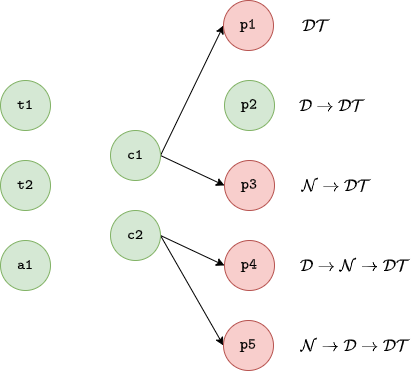
\includegraphics[width=0.45\textwidth]{img/problem_graph.png}
    \caption{Example of a Problem Graph. Green nodes are valid arguments, red ones are refuted.}
    \label{fig:pb_graph}
\end{figure}

In the last paragraphs we identified two main requirements for a human-centric framework (i.e., structure the DS knowledge in a well-defined AutoML search space, and provide the solutions in accordance with the input knowledge).
We also introduced Computational Logic -- Argumentation in particular -- as the main tool in our investigation.
Let us now delve into details of how these pieces converge in our framework.
%It is now time to show how these ideas converge in our framework.

\Cref{fig:approach} illustrates a scheme of HAMLET.
%Let us delve into details by following the CRISP-DM process flow.
The DS conducts the stages from Domain \& Data Understanding to Data Pre-processing \& Modelling, and thus gathers all the constraints that represent the knowledge discovered so far.
The Logical Knowledge Base (LogicalKB) provides a vehicle to encode such constraints.
In particular, the DS leverages an intuitive logical language, and enlists the constraints one-by-one.
In \Cref{logic} we introduced the notion of Structured Argumentation as a formal tool to convert elements from a logical language into an Argumentation graph.
Implementing and exploiting such a Structured Argumentation tool, HAMLET proceeds to resolve conflicts in the LogicalKB: the logical-encoded knowledge is transformed in a Problem Graph.%, that is then evaluated to determine possible inconsistencies in the input knowledge.
%\jg{I would drop these three following sentences}
%At the centre we find the DS. 
%She interacts with both the Knowledge Base and the Problem Graph.
%The former offers a common interface for encoding the knowledge discovered so far, while the latter a visual global overview of it---highlighting concordant and discordant insights.

%The DS can then consult the Problem Graph, outcome of this process.
The benefit of the Problem Graph is two-fold.
First of all, it can be leveraged by both the DS and Domain Experts to understand and summarise the current knowledge.
Second of all, thanks to its nature, it is straightforward to convert such a graph of constraints into a space of possible solutions (i.e., exploiting Argumentation semantics, it is easy to obtain all the sets of arguments -- constraints -- which hold together).
As a matter of fact, this feature would relieve the DS of the burden of manually considering all the effects of the possible constraints.
It is important to notice that, although the increased degree of automatisation, the Problem Graph allows the DS and Domain Experts to correct, revise, and supervise the process.
Accordingly, possible inconsistencies -- due to diverging constraints -- can be verified by the DS using her knowledge.
%Indeed, among all the benefits, it is possible to consider and visualise all the effects of the decisions with a human-readable medium.

Once the knowledge has been accurately revised, an AutoML tool is leveraged to automatise the ML pipeline instantiation.
Throughout the exploration, different solutions are tested, which contribute to augment the global knowledge about the problem.
%Most of all, several constraints -- that the DS might not have considered in the process -- are disclosed.
%In other words, AutoML receives a search space in input, which is explored, evaluated, and therefore populated.
%The new insights are useful information to .
Accordingly, some of the originally encoded knowledge by the DS and Domain Experts might be refuted or found inconsistent. %---w.r.t. some of the AutoML solutions.
%The solutions of a search space intrinsic belong to the ilk search space that should be explored.
HAMLET is designed to enable a transparent augmentation of the knowledge in the Problem Graph according to the newfound solutions.
The updating procedure is the same as the one employed by the DS during the constraint encoding phase.
Specifically, the AutoML solutions are automatically transposed to our logical language in the form of new constraints, and then added to the LogicalKB.
Of course, a change in the LogicalKB translates in a change in the Problem Graph, allowing the DS and Domain Experts to visualise and \textit{argue} about it.
The revision of the Graph is the key element in the process of augmenting the knowledge: the DS and Domain Experts can consult each other and discuss how the new insights relate with their initial knowledge.
Indeed, thanks to the nature of the Problem Graph, it would be extremely easy to identify new possible conflicts and supporting arguments.
Consequently, new constraints can be derived.

\begin{example}
In \Cref{ex:constraints} we introduce two possible ML constraints.
We now provide their encoding in the LogicalKB, and the resulting Problem Graph.
For the sake of clarity, we focus only on Discretisation ($\mathcal{D}$) and Normalisation ($\mathcal{N}$) as transformations, and Decision Tree ($\mathcal{DT}$) as the ML algorithm.
\Cref{ls:theory} contains the LogicalKB expressed in a logic language: \texttt{t1} and \texttt{t2} represent $\mathcal{D}$ and $\mathcal{N}$ respectively, \texttt{a1} represents $\mathcal{DT}$.
We consider the algorithms-related constraint \texttt{c1}, namely ``require $\mathcal{D}$ when applying $\mathcal{DT}$'', and the trnasformation-related constraint \texttt{c2}, that is ``no $\mathcal{N}$ in pipelines with $\mathcal{D}$''.
This LogicalKB is used to generate the Problem Graph shown in \Cref{fig:pb_graph}, nodes represent arguments and edges represent attacks among them.
There are five possible ML pipelines: $\mathcal{DT}$ (\texttt{p1}),  $\mathcal{D} \rightarrow \mathcal{DT}$ (\texttt{p2}),  $\mathcal{N} \rightarrow \mathcal{DT}$ (\texttt{p3}),  $\mathcal{D} \rightarrow \mathcal{N} \rightarrow \mathcal{DT}$ (\texttt{p4}), $\mathcal{N} \rightarrow \mathcal{D} \rightarrow \mathcal{DT}$ (\texttt{p5}).
With no constraints, we cannot discard any ML pipeline (i.e., there are no incompatibilities between the arguments).
By introducing \texttt{c1}, attacks against \texttt{p1} and \texttt{p3} are generated (both pipelines contain $\mathcal{DT}$ but not $\mathcal{D}$).
By introducing \texttt{c2}, attacks against \texttt{p4} and \texttt{p5} are generated (both pipelines contain $\mathcal{D}$ and $\mathcal{N}$).
We can leverage a standard argumentation semantics (e.g., Dung's grounded semantics \cite{Dung1995abstractArg}) to evaluate the graph.
In our case, all the arguments with no attacks are admissible.
Among them, we retrieve the ones representing pipelines.
\texttt{p2} is the only valid pipeline, and it will be used to generate the AutoML search space.
\label{ex:theory}
\end{example}

\Cref{ex:theory} illustrates how HAMLET leverages Logic and Argumentation to handle the DS knowledge.
The proposed logic formalism allows to easily encode the different ML constraints into a LogicalKB.
We highlight that the Problem Graph generation is handled by an argumentation engine, which is available in the Supplementary Material \footnote{\url{https://queueinc.github.io/HAMLET-DATAPLAT2022/}}.
The use of the Problem Graph allows to prune the considered ML pipeline for the AutoML search space.
AutoML could update the Problem Graph by extracting constraints from the performed exploration, and transposing them into the LogicalKB.
For instance, the DS may not have considered that data at hand contain missing values.
AutoML could help in identifying transformation-related constraints such as: ``require Imputation ($\mathcal{I}$) in all the pipelines''.
The resulting constraints might be in conflict with the previous knowledge.
In our vision, the DS is able to visualise such inconsistencies through the Problem Graph, and resolve them.

We remark how our framework is compliant with the iterative nature of the CRISP-DM standard process model.
%We already showed the iterative nature of the CRISP-DM process model.
This aspect is crucial when trying to solve real-case problems through the use of modern data platforms.
Indeed, not only the different CRISP-DM stages can be executed several times, but the whole process can be iterated, bringing new information about the problem.
We claim that our framework support and ease the adoption of the described resolution process model, by providing a tool that is both human- and machine-readable.
The knowledge can be automatically handled throughout iterations, supporting the DS in the whole analysis, in a continuous revision of the problem constraints.
At each iteration, a portion of the knowledge is known and other is discovered.
Its integration into a unified augmented knowledge graph allows to: \textit{i)} derive new constraints from the discovered knowledge, \textit{ii)} jgc{}{seamlessly} visualise possible inconsistencies and conflicts.
This naturally leads to a new iteration based on the new augmented knowledge.
Besides, the entire process might be boosted with the aid of an external knowledge.
In our vision, the DS community could create a shared LogicalKB derived from the available literature and similar real-case problems.

%%%%%%%%%%%%%%%%%%%%%%%%%%%%%%%%%%%%%%%%%%%%%%%%%%%%%%%%%%%
\section{Conclusions and potential leveraging}\label{concl}
%%%%%%%%%%%%%%%%%%%%%%%%%%%%%%%%%%%%%%%%%%%%%%%%%%%%%%%%%%%

The increasing complexity in the state-of-the-art AutoML tools has led the DS to lose the control over the resolution process.
We believe that human awareness about all the constraints and possible solutions of a ML problem is a fundamental aspect to consider, and consequently should play a key role in the design of next-generation data platforms.
Accordingly, in this vision paper we present HAMLET, a human-centric AutoML framework based on Logic and Structured Argumentation.
Logic is exploited to give a structure to the knowledge that the DS has to consider while deploying a solution.
The advantage of such a choice is twofold.
First of all, the logical encoding of the knowledge allows an easy exploration and verification of all the constraints that may apply to the case at hand---it is overwhelming for the DS to correctly handle the vast amount of them.
Second of all, it provides a medium that is both human- and machine- readable. 
The DS and Domain experts can revise the knowledge, as well as the AutoML tool, thus creating a constant feedback cycle.
We further remark that our framework could be able to address a wide range of AutoML-related challenges. 
We already highlighted a few of them: the embodiment of both ethical and legal constraints, and the construction of a shared knowledge among the DS community.

The road for future expansions is straightforward: we plan to extend this work providing a sound formalisation of HAMLET, and then a working implementation.
It will be then possible to effectively quantify the benefits of our framework and test its efficacy on real-case problems.

% \bibliographystyle{ACM-Reference-Format}
\bibliographystyle{elsarticle-num} 
\bibliography{refs}

\end{document}
\endinput
